\section{Preparation of the classification rules}

\subsection{Logistic regression}
The \verb|glm()| function in R uses the coefficients of the model to make predictions about the response variable. The \verb|glm()| function fits a generalized linear model, which is a type of statistical model that allows you to model the relationship between a response variable and one or more predictor variables.
\\\\
The \verb|glm()| function estimates the coefficients of the model by maximizing the likelihood of the data given the model. The likelihood is a measure of how well the model fits the data. The \verb|glm()| function estimates the coefficients such that the likelihood is maximized.
\\\\
Once the coefficients of the model have been estimated, the \verb|glm()| function can use them to make predictions about the response variable. Specifically, the \verb|glm()| function uses the coefficients to calculate the predicted value of the response variable for a given set of predictor variables.
\\\\
It is important to select the relevant column to have a good model. In our case, we decided to keep all the variables because looking at the figure \ref{fig:scatterplot}, all variables separate the binary indicator in 2 distinct areas.

\begin{table}[H]
\centering
\begin{tabular}{lllll}
\hline
\multicolumn{1}{|l|}{GLM} & \multicolumn{1}{l|}{Intercept}            & \multicolumn{1}{l|}{radius\_mean}     & \multicolumn{1}{l|}{texture\_mean}     & \multicolumn{1}{l|}{perimeter\_mean} \\ \hline
\multicolumn{1}{|l|}{}    & \multicolumn{1}{l|}{-18.1368587}          & \multicolumn{1}{l|}{1.3499735}        & \multicolumn{1}{l|}{0.4830149}         & \multicolumn{1}{l|}{-0.6073519}      \\ \hline
                          &                                           &                                       &                                        &                                      \\ \hline
\multicolumn{1}{|l|}{GLM} & \multicolumn{1}{l|}{area\_mean}           & \multicolumn{1}{l|}{smoothness\_mean} & \multicolumn{1}{l|}{compactness\_mean} & \multicolumn{1}{l|}{concavity\_mean} \\ \hline
\multicolumn{1}{|l|}{}    & \multicolumn{1}{l|}{0.0441134}            & \multicolumn{1}{l|}{70.3754716}       & \multicolumn{1}{l|}{-11.2074699}       & \multicolumn{1}{l|}{16.9460664}      \\ \hline
                          &                                           &                                       &                                        &                                      \\ \hline
\multicolumn{1}{|l|}{GLM} & \multicolumn{1}{l|}{concave.points\_mean} & \multicolumn{1}{l|}{symmetry\_mean}   & fractal\_dimension\_mean               & \multicolumn{1}{l|}{}                \\ \hline
\multicolumn{1}{|l|}{}    & \multicolumn{1}{l|}{76.4346011}           & \multicolumn{1}{l|}{18.9287531}       & 48.8811318                             & \multicolumn{1}{l|}{}                \\ \hline
\end{tabular}
\caption{GLM coefficients}
\label{tab:coefs_glm}
\end{table}

This gives us the following model :
\begin{align*}
    \text{pred} &= g^{-1}\mathbf{X}\beta\\
    &=g^{-1}(-18.1368587 + 1.3499735 \times \text{radius\_mean} + 0.4830149 \times \text{texture\_mean}\\
    &+ ... + 48.8811318 \times \text{fractal\_dimension\_mean})
\end{align*}

\subsection{LDA}
Linear Discriminant Analysis (LDA) is a classification algorithm that is used to predict the class label of a sample based on its features. It is a supervised learning algorithm that assumes that the features follow a Gaussian distribution within each class.
\\\\
To classify a sample using LDA, the algorithm estimates the class-conditional probability density functions (PDFs) for each class based on the training data. The class-conditional PDFs are modeled as multivariate normal distributions with class-specific means and a common covariance matrix.
\\\\
Given a new sample, LDA computes the posterior probabilities of the sample belonging to each class using Bayes' theorem. The posterior probability for each class is calculated as the product of the prior probability of the class and the likelihood of the sample belonging to the class, normalized by the sum of the likelihoods over all classes.
\\\\
The class label with the highest posterior probability is then assigned to the sample. In other words, LDA assigns the sample to the class that has the highest probability of generating the sample's features, given the class labels.
\\\\
Using all the quantitative variables, the LDA procedure
resulted in the most discriminant direction described by the coefficients in the following table :
\begin{table}[H]
\begin{tabular}{lllll}
\hline
\multicolumn{1}{|l|}{LD1} & \multicolumn{1}{l|}{radius\_mean}     & \multicolumn{1}{l|}{texture\_mean}     & \multicolumn{1}{l|}{perimeter\_mean}          & \multicolumn{1}{l|}{area\_mean}           \\ \hline
\multicolumn{1}{|l|}{}    & \multicolumn{1}{l|}{3.023569425}      & \multicolumn{1}{l|}{0.113449782}       & \multicolumn{1}{l|}{-0.363161854}             & \multicolumn{1}{l|}{-0.004811602}         \\ \hline
                          &                                       &                                        &                                               &                                           \\ \hline
\multicolumn{1}{|l|}{LD1} & \multicolumn{1}{l|}{smoothness\_mean} & \multicolumn{1}{l|}{compactness\_mean} & \multicolumn{1}{l|}{concavity\_mean}          & \multicolumn{1}{l|}{concave.points\_mean} \\ \hline
\multicolumn{1}{|l|}{}    & \multicolumn{1}{l|}{1.120549699}      & \multicolumn{1}{l|}{-0.528340038}      & \multicolumn{1}{l|}{6.051544650}              & \multicolumn{1}{l|}{29.491683288}         \\ \hline
                          &                                       &                                        &                                               &                                           \\ \hline
\multicolumn{1}{|l|}{LD1} & \multicolumn{1}{l}{symmetry\_mean}   & \multicolumn{1}{l|}{}                  & \multicolumn{1}{l}{fractal\_dimension\_mean} & \multicolumn{1}{l|}{}                     \\ \hline
\multicolumn{1}{|l|}{}    & \multicolumn{2}{l|}{6.936328511}                                               & \multicolumn{2}{l|}{13.254548376}                                                         \\ \hline
\end{tabular}
\label{tab:LDA_coef}
\caption{LDA1 coefficients}
\end{table}

This gives us the following model : 
$$\text{pred} = 3.023 \times \text{radius\_mean} + 0.1134 \times \text{texture\_mean}+ ... + 13.2445 \times \text{fractal\_dimension\_mean}$$

When we use all the variables, we have a discriminant power of $-0.8025743$. The power is negative, which means that the model is more accurate on the "malignant" cases.

\begin{table}[H]
\centering
\begin{tabular}{lllll}
\hline
\multicolumn{1}{|l|}{LD1} & \multicolumn{1}{l|}{radius\_mean}     & \multicolumn{1}{l|}{texture\_mean}     & \multicolumn{1}{l|}{perimeter\_mean} & \multicolumn{1}{l|}{area\_mean}           \\ \hline
\multicolumn{1}{|l|}{}    & \multicolumn{1}{l|}{3.042813457}      & \multicolumn{1}{l|}{0.113662563}       & \multicolumn{1}{l|}{-0.376842430}    & \multicolumn{1}{l|}{-0.004409713}         \\ \hline
                          &                                       &                                        &                                      &                                           \\ \hline
\multicolumn{1}{|l|}{LD1} & \multicolumn{1}{l|}{smoothness\_mean} & \multicolumn{1}{l|}{compactness\_mean} & \multicolumn{1}{l|}{concavity\_mean} & \multicolumn{1}{l|}{concave.points\_mean} \\ \hline
\multicolumn{1}{|l|}{}    & \multicolumn{1}{l|}{4.935756229}      & \multicolumn{1}{l|}{3.160583782}       & \multicolumn{1}{l|}{6.091609258}     & \multicolumn{1}{l|}{29.667446169}         \\ \hline
\end{tabular}
\caption{LDA without useless columns}
\label{tab:LDA2}
\end{table}
This gives us the following model : 
\begin{align*}
    \text{pred}
    &=3.043 \times \text{radius\_mean} + 0.1137 \times \text{texture\_mean}\\
    &+ ... + 69.667 \times \text{concave.points\_mean}
\end{align*}
By removing the 2 columns "symmetry\_mean" and "fractal\_dimension\_mean" we have a discriminant score of $-0.7978517$ which is better than in the previous case. \\
We chose these two column by looking at the figure \ref{fig:scatterplot} and looking for the variables the less correlated.
\subsection{ROC}
By computing the scores of each of the 2 chosen models thanks to the \verb|pROC| package, we get these ROC curves :
\begin{figure}[H]
    \centering
    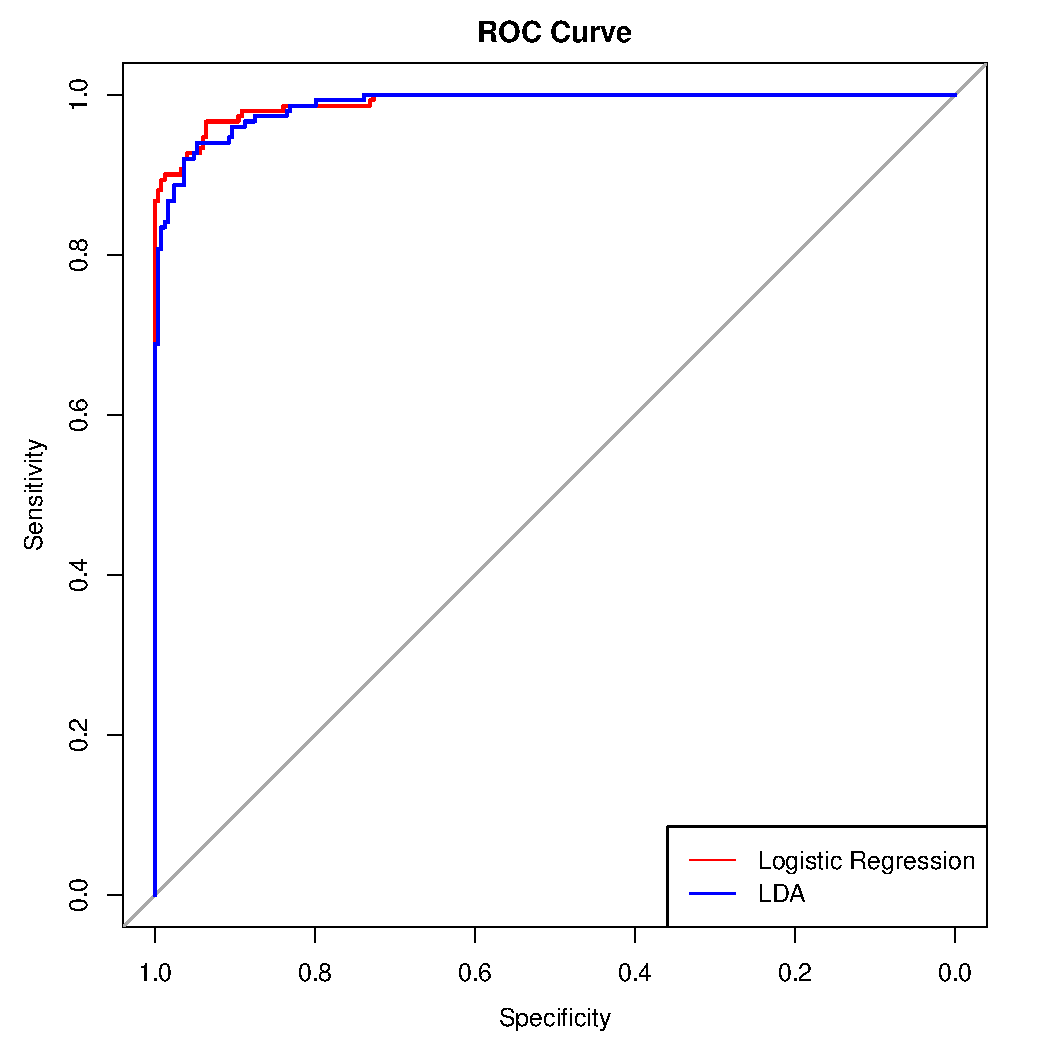
\includegraphics[width=0.5\textwidth]{figs/q2_roc.pdf}
    \caption{ROC curves}
    \label{fig:roc}
\end{figure}

The areas under the curves for GLM and LDA are respectively $0.99$ and $0.98$. We can than compute our threshold using the Youden index, for GLM and LDA respectively, these thresholds are $0.2952$ and $0.7032$.